\documentclass[
	fontsize=12pt,           % Leitlinien sprechen von Schriftgröße 12.
	paper=A4,
	twoside=false,
	listof=totoc,            % Tabellen- und Abbildungsverzeichnis ins Inhaltsverzeichnis
	bibliography=totoc,      % Literaturverzeichnis ins Inhaltsverzeichnis aufnehmen
	titlepage,               % Titlepage-Umgebung anstatt \maketitle
	headsepline,             % horizontale Linie unter Kolumnentitel
	abstract,              % Überschrift einschalten, Abstract muss in {abstract}-Umgebung stehen
]{scrreprt}                  % Verwendung von KOMA-Report
\usepackage[utf8]{inputenc}  % UTF8 Encoding einschalten
\usepackage[ngerman]{babel}  % Neue deutsche Rechtschreibung
\usepackage[T1]{fontenc}     % Ausgabe von westeuropäischen Zeichen (auch Umlaute)
\usepackage{microtype}       % Trennung von Wörtern wird besser umgesetzt
\usepackage{lmodern}         % Nicht-gerasterte Schriftarten (bei MikTeX erforderlich)
\usepackage{graphicx}        % Einbinden von Grafiken erlauben
\usepackage{wrapfig}         % Grafiken fließend im Text
\usepackage{setspace}        % Zeilenabstand \singlespacing, \onehalfspaceing, \doublespacing
\usepackage[
	%showframe,                % Ränder anzeigen lassen
	left=2.7cm, right=2.5cm,
	top=2.5cm,  bottom=2.5cm,
	includeheadfoot
]{geometry}                      % Seitenlayout einstellen
\usepackage{scrlayer-scrpage}    % Gestaltung von Fuß- und Kopfzeilen
\usepackage{acronym}             % Abkürzungen, Abkürzungsverzeichnis
\usepackage{titletoc}            % Anpassungen am Inhaltsverzeichnis
\contentsmargin{0.75cm}          % Abstand im Inhaltsverzeichnis zw. Punkt und Seitenzahl
\usepackage{newfloat}
\DeclareFloatingEnvironment[fileext=frm,placement={!ht},name=Code-Ausschnitt]{listing}
%\captionsetup[listing]{labelfont=bf}
\usepackage[                     % Klickbare Links (enth. auch "nameref", "url" Package)
  hidelinks,                     % Blende die "URL Boxen" aus.
  breaklinks=true                % Breche zu lange URLs am Zeilenende um
]{hyperref}
\usepackage[hypcap=true]{caption}% Anker Anpassung für Referenzen
\usepackage{subcaption}
\urlstyle{same}                  % Aktuelle Schrift auch für URLs
% Anpassung von autoref für Gleichungen (ergänzt runde Klammern) und Algorithm.
% Anstatt "Listing" kann auch z.B. "Code-Ausschnitt" verwendet werden. Dies sollte
% jedoch synchron gehalten werden mit \lstlistingname (siehe weiter unten).
\addto\extrasngerman{%
	\def\equationautorefname~#1\null{Gleichung~(#1)\null}
	\def\lstnumberautorefname{Zeile}
	\def\lstlistingautorefname{Listing}
	\def\algorithmautorefname{Algorithmus}
	% Damit einheitlich "Abschnitt 1.2[.3]" verwendet wird und nicht "Unterabschnitt 1.2.3"
	\def\subsectionautorefname{Abschnitt}
}

% ---- Abstand verkleinern von der Überschrift 
\renewcommand*{\chapterheadstartvskip}{\vspace*{.5\baselineskip}}

% Hierdurch werden Schusterjungen und Hurenkinder vermieden, d.h. einzelne Wörter
% auf der nächsten Seite oder in einer einzigen Zeile.
% LaTeX kann diese dennoch erzeugen, falls das Layout ansonsten nicht umsetzbar ist.
% Diese Werte sind aber gute Startwerte.
\widowpenalty10000
\clubpenalty10000


% ---- Für das Quellenverzeichnis
\usepackage[
	backend = biber,                % Verweis auf biber
	language = auto,
	style = authoryear,                % Nummerierung der Quellen mit Zahlen
	sorting = nyt,                 % none = Sortierung nach der Erscheinung im Dokument
	sortcites = true,               % Sortiert die Quellen innerhalb eines cite-Befehls
	block = space,                  % Extra Leerzeichen zwischen Blocks
	hyperref = true,                % Links sind klickbar auch in der Quelle
	%backref = true,                % Referenz, auf den Text an die zitierte Stelle
	bibencoding = auto,
	giveninits = true,              % Vornamen werden abgekürzt
	doi=true,                      % DOI nicht anzeigen
	isbn=true,                     % ISBN nicht anzeigen
    alldates=short                  % Datum immer als DD.MM.YYYY anzeigen
]{biblatex}
\addbibresource{Inhalt/literatur.bib}
\setcounter{biburlnumpenalty}{3000}     % Umbruchgrenze für Zahlen
\setcounter{biburlucpenalty}{6000}      % Umbruchgrenze für Großbuchstaben
\setcounter{biburllcpenalty}{9000}      % Umbruchgrenze für Kleinbuchstaben
\DeclareNameAlias{default}{family-given}  % Nachname vor dem Vornamen
\AtBeginBibliography{\renewcommand{\multinamedelim}{\addslash\space
}\renewcommand{\finalnamedelim}{\multinamedelim}}  % Schrägstrich zwischen den Autorennamen
\DefineBibliographyStrings{german}{
  urlseen = {Einsichtnahme:},                      % Ändern des Titels von "besucht am"
}
\usepackage[babel,german=quotes]{csquotes}         % Deutsche Anführungszeichen + Zitate

% ---- Für Mathevorlage
\usepackage{amsmath}    % Erweiterung vom Mathe-Satz
\usepackage{amssymb}    % Lädt amsfonts und weitere Symbole
\usepackage{MnSymbol}   % Für Symbole, die in amssymb nicht enthalten sind.


% ---- Für Quellcodevorlage
\usepackage{scrhack}                    % Hack zur Verw. von listings in KOMA-Script
\usepackage{listings}                   % Darstellung von Quellcode
\lstset{escapeinside={<@}{@>}}
\usepackage{xcolor}                     % Einfache Verwendung von Farben
%% -- Eigene Farben für den Quellcode
\definecolor{JavaLila}{rgb}{0.4,0.1,0.4}
\definecolor{JavaGruen}{rgb}{0.3,0.5,0.4}
\definecolor{JavaBlau}{rgb}{0.0,0.0,1.0}
\definecolor{ABAPKeywordsBlue}{HTML}{6000ff}
\definecolor{ABAPCommentGrey}{HTML}{808080}
\definecolor{ABAPStringGreen}{HTML}{4da619}
\definecolor{PyKeywordsBlue}{HTML}{0000AC}
\definecolor{PyCommentGrey}{HTML}{808080}
\definecolor{PyStringGreen}{HTML}{008080}
% -- Farben für ABAP CDS
\definecolor{CDSString}{HTML}{FF8C00}
\definecolor{CDSKeywords}{HTML}{6000ff}
\definecolor{CDSAnnotation}{HTML}{00BFFF}
\definecolor{CDSComment}{HTML}{808080}
\definecolor{CDSFunc}{HTML}{FF0000}

% -- Default Listing-Styles

\lstset{
	% Das Paket "listings" kann kein UTF-8. Deswegen werden hier 
	% die häufigsten Zeichen definiert (ä,ö,ü,...)
	literate=%
		{á}{{\'a}}1 {é}{{\'e}}1 {í}{{\'i}}1 {ó}{{\'o}}1 {ú}{{\'u}}1
		{Á}{{\'A}}1 {É}{{\'E}}1 {Í}{{\'I}}1 {Ó}{{\'O}}1 {Ú}{{\'U}}1
		{à}{{\`a}}1 {è}{{\`e}}1 {ì}{{\`i}}1 {ò}{{\`o}}1 {ù}{{\`u}}1
		{À}{{\`A}}1 {È}{{\'E}}1 {Ì}{{\`I}}1 {Ò}{{\`O}}1 {Ù}{{\`U}}1
		{ä}{{\"a}}1 {ë}{{\"e}}1 {ï}{{\"i}}1 {ö}{{\"o}}1 {ü}{{\"u}}1
		{Ä}{{\"A}}1 {Ë}{{\"E}}1 {Ï}{{\"I}}1 {Ö}{{\"O}}1 {Ü}{{\"U}}1
		{â}{{\^a}}1 {ê}{{\^e}}1 {î}{{\^i}}1 {ô}{{\^o}}1 {û}{{\^u}}1
		{Â}{{\^A}}1 {Ê}{{\^E}}1 {Î}{{\^I}}1 {Ô}{{\^O}}1 {Û}{{\^U}}1
		{œ}{{\oe}}1 {Œ}{{\OE}}1 {æ}{{\ae}}1 {Æ}{{\AE}}1 {ß}{{\ss}}1
		{ű}{{\H{u}}}1 {Ű}{{\H{U}}}1 {ő}{{\H{o}}}1 {Ő}{{\H{O}}}1
		{ç}{{\c c}}1 {Ç}{{\c C}}1 {ø}{{\o}}1 {å}{{\r a}}1 {Å}{{\r A}}1
		{€}{{\euro}}1 {£}{{\pounds}}1 {«}{{\guillemotleft}}1
		{»}{{\guillemotright}}1 {ñ}{{\~n}}1 {Ñ}{{\~N}}1 {¿}{{?`}}1,
	breaklines=true,        % Breche lange Zeilen um 
	breakatwhitespace=true, % Wenn möglich, bei Leerzeichen umbrechen
	% Symbol für Zeilenumbruch einfügen
	prebreak=\raisebox{0ex}[0ex][0ex]{\ensuremath{\rhookswarrow}},
	postbreak=\raisebox{0ex}[0ex][0ex]{\ensuremath{\rcurvearrowse\space}},
	tabsize=4,                                 % Setze die Breite eines Tabs
	basicstyle=\ttfamily\small,                % Grundsätzlicher Schriftstyle
	columns=fixed,                             % Besseres Schriftbild
	numbers=left,                              % Nummerierung der Zeilen
	%frame=single,                             % Umrandung des Codes
	showstringspaces=false,                    % Keine Leerzeichen hervorheben
	keywordstyle=\color{blue},
	ndkeywordstyle=\bfseries\color{darkgray},
	identifierstyle=\color{black},
	commentstyle=\itshape\color{JavaGruen},   % Kommentare in eigener Farbe
	stringstyle=\color{JavaBlau},             % Strings in eigener Farbe,
	captionpos=b,                             % Bild*unter*schrift
	xleftmargin=5.0ex
}

% ---- Eigener JAVA-Style für den Quellcode
\renewcommand{\ttdefault}{pcr}               % Schriftart, welche auch fett beinhaltet
\lstdefinestyle{EigenerJavaStyle}{
	language=Java,                             % Syntax Highlighting für Java
	%frame=single,                             % Umrandung des Codes
	keywordstyle=\bfseries\color{JavaLila},    % Keywords in eigener Farbe und fett
	commentstyle=\itshape\color{JavaGruen},    % Kommentare in eigener Farbe und italic
	stringstyle=\color{JavaBlau}               % Strings in eigener Farbe
}

% ---- Eigener ABAP-Style für den Quellcode
\renewcommand{\ttdefault}{pcr}
\lstdefinestyle{EigenerABAPStyle}{
	language=[R/3 6.10]ABAP,
	morestring=[b]\|,                          % Für Pipe-Strings
	morestring=[b]\`,                          % für Backtick-Strings
	keywordstyle=\bfseries\color{ABAPKeywordsBlue},
	commentstyle=\itshape\color{ABAPCommentGrey},
	stringstyle=\color{ABAPStringGreen},
	tabsize=2,
	morekeywords={
		types,
		@data,
		as,
		lower,
		start,
		selection,
		order,
		by,
		inner,
		join,
		key,
		end,
		cast
	}
}

% ---- Eigener Python-Style für den Quellcode
\renewcommand{\ttdefault}{pcr}
\lstdefinestyle{EigenerPythonStyle}{
	language=Python,
	columns=flexible,
	keywordstyle=\bfseries\color{PyKeywordsBlue},
	commentstyle=\itshape\color{PyCommentGrey},
	stringstyle=\color{PyStringGreen}
}

%----- ABAP-CDS-View language
\lstdefinelanguage{ABAPCDS}{
	sensitive=false,
	%Keywords
	morekeywords={define,
		view,
		as,
		select,
		from,
		inner,
		join,
		on,
		key,
		case,
		when,
		then,
		else,
		end,
		true,
		false,
		cast,
		where,
		and,
		distinct,
		group,
		by,
		having,
		min,
		sum,
		max,
		count,
		avg
	},
	%Methoden
	morekeywords=[2]{
		div,
		currency\_conversion,
		dats\_days\_between,
		concat\_with\_space,
		dats\_add_days,
		dats\_is\_valid,
		dats\_add\_months,
		unit\_conversion,
		division,
		mod,
		abs,
		floor,
		ceil,
		round,
		concat,
		replace,
		substring,
		left,
		right,
		length
	},
	morecomment=[s][\color{CDSAnnotation}]{@}{:},
	morecomment=[l][\itshape\color{CDSComment}]{//},
	morecomment=[s][\itshape\color{CDSComment}]{/*}{*/},
	morestring=[b][\color{CDSString}]',
	keywordstyle=\bfseries\color{CDSKeywords},
	keywordstyle=[2]\color{CDSFunc}
}

  % Weitere Details sind ausgelagert

\usepackage{algorithm}                  % Für Algorithmen-Umgebung (ähnlich wie lstlistings Umgebung)
\usepackage{algpseudocode}              % Für Pseudocode. Füge "[noend]" hinzu, wenn du kein "endif",
                                        % etc. haben willst.

\makeatletter                           % Sorgt dafür, dass man @ in Namen verwenden kann.
                                        % Ansonsten gibt es in der nächsten Zeile einen Compilefehler.
\renewcommand{\ALG@name}{Algorithmus}   % Umbenennen von "Algorithm" im Header der Listings.
\makeatother                            % Zeichen wieder zurücksetzen
\renewcommand{\lstlistingname}{Listing} % Erlaubt das Umbenennen von "Listing" in anderen Titel.

% ---- Tabellen
\usepackage{booktabs}  % Für schönere Tabellen. Enthält neue Befehle wie \midrule
\usepackage{multirow}  % Mehrzeilige Tabellen
\usepackage{siunitx}   % Für SI Einheiten und das Ausrichten Nachkommastellen
\sisetup{locale=DE, range-phrase={~bis~}, output-decimal-marker={,}} % Damit ein Komma und kein Punkt verwendet wird.
\usepackage{xfrac} % Für siunitx Option "fraction-function=\sfrac"

% ---- Für Definitionsboxen in der Einleitung
\usepackage{amsthm}                     % Liefert die Grundlagen für Theoreme
\usepackage[framemethod=tikz]{mdframed} % Boxen für die Umrandung
% ------ Definition zum Strich vor eines Texts
\newmdtheoremenv[
  hidealllines = true,       % Rahmen komplett ausblenden
  leftline = true,           % Linie links einschalten
  innertopmargin = 0pt,      % Abstand oben
  innerbottommargin = 4pt,   % Abstand unten
  innerrightmargin = 0pt,    % Abstand rechts
  linewidth = 3pt,           % Linienbreite
  linecolor = gray!40,       % Linienfarbe
]{defStrich}{Definition}     % Name der des formats "defStrich"

% ------ Definition zum Eck-Kasten um einen Text
\newmdtheoremenv[
  hidealllines = true,
  innertopmargin = 6pt,
  linecolor = gray!40,
  singleextra={              % Eck-Markierungen für die Definition
    \draw[line width=3pt,gray!50,line cap=rect] (O|-P) -- +(1cm,0pt);
    \draw[line width=3pt,gray!50,line cap=rect] (O|-P) -- +(0pt,-1cm);
    \draw[line width=3pt,gray!50,line cap=rect] (O-|P) -- +(-1cm,0pt);
    \draw[line width=3pt,gray!50,line cap=rect] (O-|P) -- +(0pt,1cm);
  }
]{defEckKasten}{Definition}  % Name der des formats "defEckKasten"

\newmdtheoremenv[
  hidealllines = true,
  leftline = true,
  innertopmargin = 0pt,
  innerbottommargin = 4pt,
  innerrightmargin = 0pt,
  linewidth = 3pt,
  linecolor = gray!40,
  ]{definition}{Definition}[]
\newcommand{\definitionautorefname}{Definition}
  % Weitere Details sind ausgelagert

% ---- Für Todo Notes
%\usepackage[disable]{todonotes}
\usepackage{todonotes}
\setlength {\marginparwidth }{2cm}

% ---- Zum Einbinden von PDF-Dokumenten
\usepackage{pdfpages}

% ---- Für Tikz
\usepackage{tikz}
\usetikzlibrary{shapes,arrows}


% ---- Elektronische Version oder Gedruckte Version?
% ---- Unterschied: Die elektronische Version enthält keinen Platzhalter für die Unterschrift
\usepackage{ifthen}
\newboolean{e-Abgabe}
\setboolean{e-Abgabe}{false}    % false=gedruckte Fassung

% ---- Persönlichen Daten:
\newcommand{\titel}{Performance Analyse der Optimierung von Datenbankabfragen in der HANA \acl{CE}}
%\newcommand{\titelheader}{Performance Messung und Optimierung in der HANA-Analytics-CalcEngine}
\newcommand{\arbeit}{Projektarbeit 2}
\newcommand{\studiengang}{Wirtschaftsinformatik}
\newcommand{\studienjahr}{2022}
\newcommand{\autor}{Jared Heinrich}
\newcommand{\autorReverse}{Heinrich, Jared}
\newcommand{\verfassungsort}{Mannheim}
\newcommand{\matrikelnr}{5101479}
\newcommand{\kurs}{WWI22SEA}
\newcommand{\bearbeitungsmonat}{August 2024}
\newcommand{\abgabe}{26. August 2024}
\newcommand{\bearbeitungszeitraum}{06.05.2024 - 25.08.2024}
\newcommand{\firmaName}{SAP SE}
\newcommand{\firmaStrasse}{Dietmar-Hopp-Allee 16}
\newcommand{\firmaPlz}{69190 Walldorf, Deutschland}
\newcommand{\betreuerFirma}{Rainer Agelek}
\newcommand{\betreuerDhbw}{Prof. Dr. Hans-Henning Pagnia}

% ---- Metainformation für das PDF Dokument
\hypersetup{
	pdftitle    = {\titel},
	pdfsubject  = {\arbeit},
	pdfauthor   = {\autor},
	%pdfkeywords = {Keywords angeben},
	pdfcreator  = {LaTeX},
	%pdfproducer = {in der Regel pdfTeX}
}

% ---- Definition der Kopf- und Fußzeilen
\clearpairofpagestyles                          % Löschen von LaTeX Standard
\automark[section]{chapter}                     % Füllen von section und chapter
\renewcommand*{\chaptermarkformat}{}            % Entfernt die Kapitelnummer
\renewcommand*{\sectionmarkformat}{}            % Entfernt die Sectionnummer
% Angaben [für "plain"]{für "scrheadings"}
%\ihead[]{\titelheader}                          % Kopfzeile links
\chead[]{}                                      % Kopfzeile mitte
\ohead[]{\rightmark}                            % Kopfzeile rechts
\ifoot[]{}                                      % Fußzeile links
\cfoot*{\sffamily\pagemark}                     % Fußzeile mitte
\ofoot[]{}                                      % Fußzeile rechts
\KOMAoptions{
   headsepline = 0.2pt,                         % Liniendicke Kopfzeile
   footsepline = false                          % Liniendicke Fußzeile
}


% ---- Hilfreiches
\newcommand{\zB}{z.\,B. }   % "z.B." mit kleinem Leeraum dazwischen (ohne wäre nicht korrekt)
\newcommand{\dash}{d.\,h. }

\newcommand{\code}[1]{\texttt{#1}} % Ist einfacher zu schreiben als ständig \texttt und erlaubt
                                   % Änderungen im Nachhinein, wenn man z.B. Inline-Code anders stylen möchte.
% ---- Silbentrennung (falls LaTeX defaults falsch / nicht gewünscht sind)
\hyphenation{HANA}         % anstatt HA-NA
\hyphenation{Graph-Script} % anstatt GraphS-cript

% ---- Beginn des Dokuments
\begin{document}
\setlength{\parindent}{0pt}              % Keine Paragraphen Einrückung.
                                         % Dafür haben wir den Abstand zwischen den Paragraphen.
\setcounter{secnumdepth}{2}              % Nummerierungstiefe fürs Inhaltsverzeichnis
\setcounter{tocdepth}{1}                 % Tiefe des Inhaltsverzeichnisses. Ggf. so anpassen,
                                         % dass das Verzeichnis auf eine Seite passt.
\sffamily                                % Serifenlose Schrift verwenden.

% ---- Vorspann
% ------ Titelseite
\singlespacing
\thispagestyle{empty}
\begin{titlepage}
\enlargethispage{4cm}

\begin{figure}           % Logo vom Ausbildungsbetrieb und der DHBW
	% \vspace*{-5mm} % Sollte dein Titel zu lang werden, kannst du mit diesem "Hack" 
	%                  den Inhalt der Seite nach oben schieben.
	\begin{minipage}{0.49\textwidth}
		\flushleft
		
\includegraphics[height=2.5cm]{Bilder/Logos/Logo_SAP.pdf} 
	\end{minipage}
	\hfill
	\begin{minipage}{0.49\textwidth}
		\flushright
		
\includegraphics[height=2.5cm]{Bilder/Logos/Logo_DHBW.pdf} 
	\end{minipage}
\end{figure} 
\vspace*{0.1cm}

\begin{center}
	\huge{\textbf{\titel}}\\[1.5cm]
	\Large{\textbf{\arbeit}}\\[0.5cm]
	\normalsize{im Rahmen der Prüfung zum\\[1ex] \textbf{Bachelor of Science (B.Sc.)}}\\[0.5cm]
	\Large{des Studienganges \studiengang}\\[1ex]
	\normalsize{an der Dualen Hochschule Baden-Württemberg Mannheim}\\[1cm]
	\normalsize{von}\\[1ex] \Large{\textbf{\autor}} \\[1cm]
	% Hinweis: Manche Dozenten möchten einen Hinweis auf den Sperrvermerk auf der Titelseite.
	% \large{{\color{red}- Sperrvermerk -}}\\[1cm]
\end{center}

\begin{center}
	\vfill
	\begin{tabular}{ll}
		Abgabedatum:                 & \abgabe \\[0.2cm]
		Bearbeitungszeitraum:        & \bearbeitungszeitraum \\[0.2cm]
		Matrikelnummer, Kurs:        & \matrikelnr  , \kurs \\[0.2cm]
		Ausbildungsfirma:            & \firmaName \\
		                             & \firmaStrasse \\
		                             & \firmaPlz \\[0.2cm]
		Unternehmensbetreuer:        & \betreuerFirma \\[0.2cm]
		Wissenschaftlicher Betreuer: & \betreuerDhbw \\[2cm]
	\end{tabular} 
\end{center}
\end{titlepage}
  % Titelseite
\newcounter{savepage}
\pagenumbering{Roman}                    % Römische Seitenzahlen
\onehalfspacing

% ------ Erklärung, Sperrvermerk, Abstact
\chapter*{Ehrenwörtliche Erklärung}

Ich versichere hiermit, dass ich die vorliegende Arbeit mit dem Thema: 

\begin{quote}
	\textit{\titel}
\end{quote} 

selbstständig
verfasst und keine anderen als die angegebenen Quellen und Hilfsmittel benutzt habe.

\vspace{0.25cm}

Ich versichere zudem, dass die eingereichte elektronische Fassung mit der gedruckten Fassung übereinstimmt.

\vspace{1cm}

\verfassungsort, den \today \\[0.5cm]
\ifthenelse{\boolean{e-Abgabe}}
	{\underline{Gez. \autor}}
	{\makebox[6cm]{\hrulefill}}\\ 
\autorReverse

\include{Standard/sperrvermerk}
\renewcommand{\abstractname}{Abstract} % Veränderter Name für das Abstract
\begin{abstract}
\begin{addmargin}[1.5cm]{1.5cm}        % Erhöhte Ränder, für Abstract Look
\thispagestyle{plain}                  % Seitenzahl auf der Abstract Seite

\begin{center}
\small\textit{- Deutsch -}             % Angabe der Sprache für das Abstract
\end{center}

\vspace{0.25cm}

%Dies ist der Beginn des Abstracts. Für die finale Bachelorarbeit musst du ein Abstract in deinem Dokument mit einbauen. So, schreibe es am besten jetzt in Deutsch und Englisch. Das Abstract ist eine kurze Zusammenfassung mit ca. 200 bis 250 Wörtern.
Das ist der Abstract.

\vspace{0.25cm}

%Versuche in das Abstract folgende Punkte aufzunehmen: Fragestellung der Arbeit, methodische Vorgehensweise oder die Hauptergebnisse deiner Arbeit.


\end{addmargin}
\end{abstract}


% ------ Inhaltsverzeichnis
\singlespacing
\tableofcontents

% ------ Verzeichnisse
\renewcommand*{\chapterpagestyle}{plain}
\pagestyle{plain}
\include{Verzeichnisse/formelgroessen}
\chapter*{Abkürzungsverzeichnis}
\addcontentsline{toc}{chapter}{Abkürzungsverzeichnis} % Hinzufügen zum Inhaltsverzeichnis 

\begin{acronym}[CE] % längstes Kürzel wird verw. für den Abstand zw. Kürzel u. Text

	% Alphabetisch selbst sortieren - nicht verwendete Kürzel rausnehmen!
	\acro{CE}{Calculation Engine}

\end{acronym}

\listoffigures                          % Erzeugen des Abbildungsverzeichnisses 
\listoftables                           % Erzeugen des Tabellenverzeichnisses
\renewcommand{\listlistingname}{Quellcodeverzeichnis}
\listoflistings
\setcounter{savepage}{\value{page}}


% ---- Inhalt der Arbeit
\cleardoublepage
\pagenumbering{arabic}                  % Arabische Seitenzahlen für den Hauptteil
\setlength{\parskip}{0.5\baselineskip}  % Abstand zwischen Absätzen
\rmfamily
\renewcommand*{\chapterpagestyle}{scrheadings}
\pagestyle{scrheadings}
\onehalfspacing
\chapter{Einleitung}

\chapter{Grundlagen}

\section{\acl{CE}}
%HANA?

\section{Modelle und Datenbankabfragen}
\label{sec:modells_db_queries}
Um Daten einer HANA Datenbank zu analysieren, können sogenannte
Kalkulationssichten genutzt werden. Da nur diese Kalkulationssichten in der
Arbeit weiter betrachtet werden, werden sie im Folgenden auch als
Datenbankabfragen bezeichnet. \autocite[Vgl.][]{SapHanaCreateCalcViews}

In der \ac{CE} werden diese Datenbankabfragen durch Modelle dargestellt. Für
jede Abfrage wird zuerst das dazugehörige Modell instanziiert. Anschließend
wird dieses Modell optimiert, um die Ausführungsdauer der Abfrage zu
minimieren.  Diese optimierte Abfrage, wird dann auf der Datenbank ausgeführt.
Allgemein kann man ein Modell als azyklischen gerichteten Graphen nach
\autoref{def:gerichteter_graph} und \autoref{def:zyklen} beschreiben. Des
Weiteren ist zu beachten, dass dieser Graph nur eine Quelle nach
\autoref{def:quelle_senke} hat, welche auch als Abfrageknoten bezeichnet wird.
Diese Definitionen reichen jedoch nicht aus, da zwischen verschiedenen Arten
von Knoten unterschieden wird, welche jeweils verschiedene Informationen
beinhalten.  Allgemein werden die Knoten in der \ac{CE} in zwei Gruppen
unterschieden, Datenquellen und Sichtknoten. Es gibt verschiedene Datenquellen,
zur Vereinfachung werden in dieser jedoch Arbeit nur
\foreignlanguage{english}{Table}-Knoten betrachtet. Deshalb werden Datenquellen
im Folgenden auch Tabellenknoten genannt.
%Ein \foreignlanguage{english}{Table}-Knoten spiegelt eine Tabelle einer Datenbank wider.
Die andere Gruppe sind die Sichtknoten. Zu diesen gehören \zB
\foreignlanguage{english}{Projection}, \foreignlanguage{english}{Aggregation},
\foreignlanguage{english}{Join} und \foreignlanguage{english}{Union}. Auch hier
gibt es zwar noch Weitere, diese Arbeit beschränkt sich jedoch auf diese.
Diese Modelle könnte man zwar wie in \autoref{def:gerichteter_graph}
beschreiben als eine Menge von Knoten und Kanten darstellen, gespeichert wird
jedoch eine Liste an Knoten, von welchen jedem seine Kind- und Elternknoten
zugeordnet sind. Die Kindknoten werden dabei als Eingangsknoten und die
Elternknoten als Ausgangsknoten bezeichnet. Jeder Knoten kann beliebig viele
Ausgangsknoten haben, wobei es wie bereits beschreiben nur einen Knoten mit $0$
Ausgangsknoten gibt. Die Anzahl der Eingangsknoten unterscheidet sich dabei je
nach Knotentyp.
\foreignlanguage{english}{Projection}- und
\foreignlanguage{english}{Aggregation}-Knoten haben genau einen, \todo{Was genau ist Aggregation}
\foreignlanguage{english}{Join}- \todo{Join nur 2}und \foreignlanguage{english}{Union}-Knoten
haben zwei oder mehr und ein \foreignlanguage{english}{Table}-Knoten hat keinen
Eingangsknoten. Bei den Eingangsknoten kann es sich um Tabellenknoten
sowie auch Sichtknoten handeln. \autocite[Vgl.][/Create Calculation
Views/Supported View Nodes for Modeling Calculation
Views]{SapHanaCreateCalcViews}

\autoref{fig:bsp_modell} zeigt ein einfaches Beispielmodell, welches zur
Veranschaulichung dient. Das Modell besteht aus fünf Knoten, dem Abfrageknoten,
zwei Sichtknoten und zwei Tabellenknoten. In dem Knoten steht der Name des
Knotens und neben ihm steht der Knotentyp. Bis auf den Abfrageknoten haben in
diesem Beispiel alle Knoten eine Zahl als Namen. Der Abfrageknoten sowie alle
Tabellenknoten sind zusätzlich farblich markiert. Knoten 1 ist ein
\foreignlanguage{english}{Join}-Knoten. Er hat zwei Eingangsknoten,
den \foreignlanguage{english}{Table}-Knoten 2 und den
\foreignlanguage{english}{Projection}-Knoten 3. Der einzige Ausgangsknoten ist in diesem Fall der
Abfrageknoten, dieser ist hier vom Typ \foreignlanguage{english}{Aggregation}.
Der Abfrageknoten könnte jedoch alternativ auch vom Typ \foreignlanguage{english}{Projection} sein. \todo{Unsicher??}

\begin{figure}
    \begin{center}
        \begin{tikzpicture}[
    node distance = 1cm,
    request/.style = {rectangle, draw, blue, minimum width=2cm, minimum height=0.8cm},
    op_node/.style = {circle, draw, minimum size=1cm},
    table_node/.style = {circle, draw, magenta, minimum size=1cm},
    arrow/.style = {->, >=stealth}
]

% Nodes
\node[request] (0) at (0,3) {Abfrage};
\node[right=0.2cm of 0] {Aggregation};

\node[op_node] (1) at (0,1) {1};
\node[below=0.2cm of 1] {Join};

\node[table_node] (2) at (-2,-1) {2};
\node[below=0.2cm of 2] {Table};

\node[op_node] (3) at (2,-1) {3};
\node[right=0.2cm of 3] {Projection};

\node[table_node] (4) at (2,-3) {4};
\node[below=0.2cm of 4] {Table};

% Arrows
\draw[arrow] (0) -- (1);
\draw[arrow] (1) to[out=210,in=90] (2);
\draw[arrow] (1) to[out=-30,in=90] (3);
\draw[arrow] (3) -- (4);

\end{tikzpicture}

    \end{center}
    \caption{Beispiel Modell}\label{fig:bsp_modell}
\end{figure}

Zusätzlich zu den Eingangs- und Ausgangsknoten werden in jedem Knoten
noch weitere Informationen gespeichert. Jeder Knoten beinhaltet
eine Liste an Sichtattributen, diese legt fest, welche Sichtattribute dieser
Knoten an seine Ausgangsknoten weitergibt. Bei einem Tabellenknoten sind die
Sichtattribute gleichbedeutend mit den Spalten der Tabelle. Die Sichtattribute
des Abfrageknotens sind die Attribute, welche im Ergebnis der Abfrage enthalten
sind. Damit Sichtattribute umbenannt werden können, wird jedem Eingangsknoten
eine Liste an Mappings zugeordnet. Hat der Knoten $N$ einen Eingangsknoten $E$
mit einem Mapping, dann bildet dieses ein Sichtattribut von $E$ auf ein
Sichtattribut von $N$ ab.

Die verschiedenen Sichtknotentypen sind für verschiedene Operationen zuständig.
Manche dieser Knoten haben noch zusätzliche Attribute, um die genaue Art und
Weise der Operation festzulegen.
Ein \foreignlanguage{english}{Join}-Knoten kann genutzt werden, um die
Ergebnisse der beiden Eingangsknoten zu verbinden. 

% section Modelle und Datenbankabfragen (end)

\section{Verschiedene Arten von Performance Analyse}
\label{sec:arten_performance_analyse}
\subsubsection*{Benchmarking}
\subsubsection*{Profiling}

% section Verschiedene Arten von Performance Analyse (end)

\section{Notwendige Grundlagen aus der Graphentheorie}
\label{sec:grundlagen_graphentheorie}

\autoref{def:gerichteter_graph} gibt eine Definition für einen gerichteten
Graphen \autocite[vgl.][220]{AlgorithmenUndDatenstrukturen}.
\begin{definition}
    Ein gerichteter Graph ist ein Tupel $G=(V,E)$. $V$ heißt Menge der Knoten.
    $E$ heißt Menge der gerichteten Kanten. Es gilt $V\ne\emptyset$ und $E \subset V \times
    V \setminus \{(v,v) | v \in V\}$. Zwischen zwei Knoten $u,v \in V$ gibt es
    eine Kante mit dem Anfangspunkt $u$ und dem Endpunkt $v$, wenn $(u,v) \in E$.
    \label{def:gerichteter_graph}
\end{definition}

\autoref{def:pfad} gibt eine Definition für einen Pfad in einem Graphen
\autocite[vgl.][221f]{AlgorithmenUndDatenstrukturen}.
\begin{definition}
    Ein Pfad $P$ in $G$  ist eine Folge von Knoten $v_0, \dots ,v_n$. Dabei
    muss $\forall i \in \{0; \dots; n-1 \} : (v_i,v_{i+1}) \in E$ gelten. $v_0$
    heißt Anfangspunkt von $P$, $v_n$ heißt Endpunkt von $P$ und $n$ heißt
    Länge von $P$.
    \label{def:pfad}
\end{definition}

\autoref{def:zyklen} gibt  eine Definition für Zyklen in einem gerichteten
Graphen und definiert den Begriff des azyklischen Graphen
\autocite[vgl.][222]{AlgorithmenUndDatenstrukturen}.
\begin{definition}
    Ein Pfad heißt geschlossen, wenn $v_0 = v_n$. Ein
    geschlossener Pfad heißt einfach, wenn $\forall i,j \in \{0; \dots; n-1\}, i
    \ne j:v_i \ne v_j$ gilt. In einem gerichteten Graphen heißt ein einfach
    geschlossener Pfad mit $n\geq 2$ auch Zyklus. Ein Graph heißt azyklisch,
    wenn er keine Zyklen besitzt.
    \label{def:zyklen}
\end{definition}

\autoref{def:gewichteter_graph} definiert den Begriff des gewichteten Graphen
\autocite[vgl.][253]{AlgorithmenUndDatenstrukturen}.
\begin{definition}
    $G$ heißt gewichtet, wenn es eine Abbildung $g:E\rightarrow \mathbb{R}$
    gibt, welche jeder Kante ein Gewicht zuordnet. Für $e\in E$ heißt $g(e)$
    Gewicht von $e$.
    \label{def:gewichteter_graph}
\end{definition}

\autoref{def:quelle_senke} definiert die Begriffe Quelle und Senke
\autocite[vgl.][306]{AlgorithmenUndDatenstrukturen}.
\begin{definition}
    Ein Knoten $q \in V$ heißt Quelle, wenn $ \forall p \in V: (p,q) \not \in E
    $, $q$ also nach \autoref{def:kind_eltern} keine Elternknoten hat.
    $s \in V$ heißt Senke, wenn $ \forall p \in V: (s,p) \not \in E $, $s$ also
    nach \autoref{def:kind_eltern} keine Kindknoten hat.
    \label{def:quelle_senke}
\end{definition}

\autoref{def:kind_eltern} definiert die Begriffe Kindknoten, Elternknoten und
Subknoten.
\begin{definition}
    Für zwei Knoten $c$ und $p$ gilt, $c$ ist Kindknoten von $p$, wenn $(p,c)\in E$.
    Umgekehrt gilt, wenn $(p,c)\in E$, $p$ ist Elternknoten von $c$.
    $c$ ist Subknoten von $p$, wenn $\exists P: (v_0=p) \land (v_n=c)$, es also
    einen Pfad von $p$ nach $c$ gibt.
    \label{def:kind_eltern}
\end{definition}
% section Notwendige Grundlagen aus der Graphentheorie (end)

\chapter{Aktueller Stand der Performance Analyse in der \acl{CE}}
\label{sec:analyse}
In der \ac{CE} werden bereits verschiedene Wege genutzt, um die Performance und
das Verhalten der HANA Datenbank zu analysieren. 
\section{Google Benchmark}
\label{sec:google_benchmark}

Google Benchmark ist ein Open Source Benchmarking Tool von Google,
welches es einem ermöglicht einzelne Funktionen in C++ zu benchmarken. 
Dazu kann man ähnlich zu den meisten Test Frameworks drei verschiedene
Codeabschnitte definieren.

Der Hauptabschnitt definiert was genau im Benchmark untersucht werden
soll. Diese legt die für die Messung relevante Logik fest.
Der Setup Abschnitt wird einmal vor jeder Ausführung des Benchmarks
aufgerufen. In dieser werden die Voraussetzungen für die Ausführung des Hauptabschnitts
geschaffen. Man könnte sie beispielsweise nutzen, um Testdaten für den Benchmark
zu generieren oder zu laden, da er nicht bei den Messungen beachtet wird.
Der Teardown Abschnitt wird nach jeder Ausführung des Benchmarks aufgerufen.
Dieser beeinflusst, wie der Setup Abschnitt, die Messung nicht.

Des Weiteren bietet Google Benchmark die Option, einen Benchmark mehrmals mit
unterschiedlichen Parametern durchzuführen. Um beispielsweise die Auswirkung
der Größe des Testdatensatzes auf das Ergebnis zu beobachten.

\autoref{fig:google_benchmark_ausgabe} zeigt eine Beispielhafte Google
Benchmark Ausgabe. Benchmark ist dabei der Name des Benchmarks und hinter dem
Schrägstrich die Größe des Inputs. \foreignlanguage{english}{Time} ist die durchschnittliche Dauer einer
Ausführung des Hauptabschnitts über alle Iterationen hinweg. CPU ist die
durchschnittliche CPU Zeit einer Ausführung des Hauptabschnitts über alle
Iterationen hinweg. \foreignlanguage{english}{Iterations} ist die Anzahl der durchgeführten Wiederholungen
des Hauptabschnitts. Legt man keine Anzahl fest, wird die Anzahl der
Wiederholungen anhand der durchschnittlichen Dauer einer Iteration und der
Varianz der Dauer über alle Iterationen hinweg festgelegt.
\autocite[Vgl.][]{GoogleBenchmark}

\begin{figure}[h]
    \begin{center}
        \begin{verbatim}

---------------------------------------------------------------
Benchmark                          Time         CPU Iterations 
---------------------------------------------------------------
BM_RemoveDetachedNodes/2           4 us        4 us     189823 
BM_RemoveDetachedNodes/8           9 us        9 us      78165 
BM_RemoveDetachedNodes/64         58 us       58 us      12106 
BM_RemoveDetachedNodes/512       469 us      468 us       1515 
BM_RemoveDetachedNodes/4096     4237 us     4234 us        166 
BM_RemoveDetachedNodes/8192    10026 us    10019 us         60 
        \end{verbatim}
    \end{center}
    \caption{Google Benchmark Ausgabe}\label{fig:google_benchmark_ausgabe}
\end{figure}

Google Benchmark wird in der \ac{CE} meistens genutzt, um das Verhalten der
Laufzeit bestimmter Funktionen in künstlich generierten Testfällen zu
vergleichen. Hierbei wird keine HANA Instanz benötigt, da
keine Operationen auf einer Datenbank ausgeführt werden, sondern nur einzelne
Funktionen aufgerufen werden. Es werden folglich
auch keine Testdatensätze für die Datenbank benötigt, sondern nur Daten, auf
welchen man die zu analysierende Funktion aufrufen kann.

Im Vergleich zu anderen Methoden der Performance Messung, die Operationen auf
einer HANA-Instanz ausführen, ist ein Google Benchmark relativ einfach.
Dies liegt daran, dass sie weniger Voraussetzungen erfordern und sich lediglich
auf einen kleinen Teil der Logik konzentrieren.
% section Google Benchmark (end)

\section{HANA Profiler}
\label{sec:hana_profiler}


Eine weitere Methode die Performance und das Verhalten von Software zu
analysieren ist, das bereits in \autoref{sec:arten_performance_analyse}
beschriebene, Profiling.

In der \ac{CE} wird hauptsächlich der \enquote{BOOSS-Profiler}, ein in HANA
integrierter Profiler, verwendet. Auf diesen kann entweder manuell oder im Code
zugegriffen werden. Dabei sind die wichtigsten Befehle \texttt{profiler clear}
um die aktuellen Profilinginformationen zurückzusetzen,  \texttt{profiler
start} um den Profiler zu starten, \texttt{profiler stop} um den Profiler zu
stoppen und \texttt{profiler print} um die gesammelten Profilinginformationen
auszugeben.

Der Profiler kann in diesem Kontext auf zwei verschiedene Arten genutzt werden.
Entweder in dem zur Laufzeit des Profilers Anfragen an eine bestehende
HANA-Instanz gestellt werden. Oder der Profiler wird innerhalb eines Tests oder
Benchmarks aufgerufen und es werden die dort aufgerufen Funktionen gemessen.

Die Ausgabe erzeugt dabei ist dabei zwei gewichtete gerichtete azyklische
Graphen, nach \autoref{sec:grundlagen_graphentheorie}, von denen einer die Verteilung der CPU-Zeit und der andere die
Verteilung der Wartezeit, der aufgerufenen Funktionen beinhaltet. Im Folgenden
werden die beiden Graphen CPU-Graph und Warte-Graph genannt.
\autoref{fig:beispielausgabe_hana_profiler} stellt eine mögliche Ausgabe des
HANA Profilers dar. Die folgende Beschreibung gilt für den CPU- als auch den
Warte-Graphen. Jeder Knoten des Graphen spiegelt eine zur Laufzeit des
Profilers aufgerufene Funktion wider. Jeder Knoten beinhaltet drei
Informationen. Den Namen der aufgerufenen Funktion, sowie den Wert $I$ und den
Wert $E$. $I$ ist der Anteil der Gesamtzeit, welcher von diesem Knoten und all
seinen Subknoten benötigt wurde. $E$ ist der Anteil der Gesamtzeit, welcher
von diesem Knoten benötigt wurde. Folglich gilt für alle Knoten $I\geq E$.
Die Kindknoten eines Knoten $K$ sind die Funktionen, welche von $K$ aufgerufen
wurden.

\begin{figure}[h]
    \begin{center}
        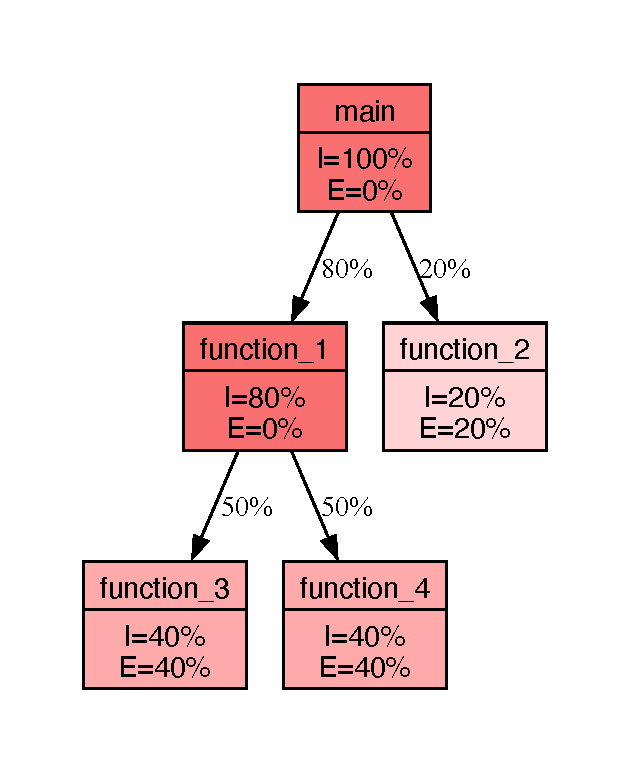
\includegraphics[page=1]{Bilder/pdf/profiler_output_example.pdf}
    \end{center}
    \caption{Beispielausgabe des HANA Profilers}\label{fig:beispielausgabe_hana_profiler}
\end{figure}

% section HANA Profiler (end)

\chapter{Konzept}

Für die Untersuchung des Optimierungsalgorithmus wird ein experimenteller
Ansatz statt einem analytischem gewählt, da die experimentelle Vorgehensweise
es zum einen einfacher macht sehr komplexe Algorithmen zu untersuchen, zum
anderen, eine experimentelle Untersuchung realitätsnähere Ergebnisse liefern
kann \autocite[vgl.][3]{ExperimentalMethods}. Hierzu werden in dieser Arbeit
zwei unabhängige Variablen betrachtet. Zum einen die Größe und zum anderen der
Aufbau des zu optimierenden Modells, diese wurden gewählt, da sie direkt
kontrolliert werden können und erwartet wird, dass sie einen großen Einfluss
auf die Laufzeit haben \autocite[vgl.][506]{ExperimentalAnalysis}. Der Aufbau
wird in dieser Arbeit als Art des Modells bezeichnet. Die gemessene abhängige
Variable ist die Laufzeit des Optimierungsvorgangs. Unabhängige Variablen sind
Variablen, welche aktiv verändert werden, während abhängige Variablen gemessen
werden \autocite[vgl.][236]{EmpirischeMethoden}. Damit Messergebnisse
sinnvoll vergleichen werden können, darf zwischen zwei Messungen nur eine
unabhängige Variable verändern werden. \autocite[vgl.][236]{EmpirischeMethoden}.
Deshalb werden mehrere Messreihen durchgeführt, wobei innerhalb einer Messreihe
der Art konstant ist, die Größe jedoch variabel ist. Für jede Art wird eine
neue Messreihe begonnen. Störvariablen, also Einflussfaktoren, welche ebenfalls
die abhängigen Variablen beeinflussen, jedoch während der Messung
unkontrolliert auftreten, \zB die Prozessorauslastung des Rechners, auf
welchem die Messung durchgeführt wird \autocite[vgl.][237]{EmpirischeMethoden}.
Ist der Prozessor weniger ausgelastet, dann ist die gemessene Zeit vermutlich
geringer, als wenn der Prozessor stark ausgelastet ist.

Um den Einfluss dieser Störvariablen möglichst gering zu halten, wird jede Messung
$n$ mal wiederholt. Aus diesen Messwerten wird nun ein Konfidenzintervall
gebildet, welches mit der Wahrscheinlichkeit $1 - \alpha$ den tatsächlichen
Erwartungswert $\mu$ enthält. Dazu werden die Messwerte als eine T-verteilte
Zufallsvariable $X$ betrachtet, da $n$ aufgrund der Dauer einer Messung nicht
sehr groß gewählt werden kann. Die Varianz $\sigma^2$ von $X$ ist dabei
unbekannt und muss anhand der Stichprobe geschätzt werden, für diese Schätzung
gilt: $\hat{\sigma}^2 = S^2$ \autocite[vgl][528]{Statistik}. Für das
($1-\alpha$)-Konfidenzintervall ergibt sich deshalb nach
\autocite[vgl.][533]{Statistik}:

\begin{equation*}
    [\bar{X} - t_{n-1,1-\alpha/2}\sqrt{S^2/n}, \bar{X} +
    t_{n-1,1-\alpha/2}\sqrt{S^2/n}]
\end{equation*}

Dabei ist $\bar{X}$ der Mittelwert der Stichprobe und $S^2$ die korrigierte
Stichprobenvarianz \autocites[vgl.][59, 502]{Statistik}. 
\begin{equation*}
    \bar{X} = \frac{1}{n} \displaystyle\sum^{n}_{i=1}x_i 
\end{equation*}
\begin{equation*}
    S^2 = \frac{1}{n-1}\displaystyle\sum^{n}_{i=1}(x_i-\bar{X})^2
\end{equation*}

Für die verschiedenen Arten von Modellen, werden Modelle, von reellen Abfragen
betrachtet, um aus diesen, allgemeine Regeln festzulegen, mit welchen man
Modelle variabler Größe aber derselben Art erzeugen kann. Die Modelle werden
für die Messung künstlich erzeugt, um die unabhängigen Variablen gezielt
verändern zu können. Auf die reellen Abfragen wird dabei zurückgegriffen, um
die Relevanz der Messung, für reelle Szenarien zu erhöhen.
\autocite[Vgl.][500f]{ExperimentalAnalysis}

Diese Messdaten werden genutzt, um festzustellen, wie sich die Laufzeit der
Optimierung für Modelle bestimmter Art bei steigender Größe verhalten. Dabei
ist besonders interessant, ob sich die Laufzeit zur Größe linear verhält,
beziehungsweise ob sie stärker oder schwächer ansteigt. Für die Optimierung des
Algorithmus sind nun die Modellarten interessant, bei welchen die Laufzeit
stärker als linear ansteigt, da diese Modellarten ein besonders hohes Potenzial
haben lange Laufzeiten zu verursachen. Um genauer herauszufinden, in welchem
Teil des Optimierungsalgorithmus besonders viel Zeit benötigt wurde, werden
diese Modelle nochmals mithilfe des in \autoref{sec:performance_analyse}
beschriebenen Profilings untersucht.
Dazu werden mehrere Modelle dieser Art
optimiert, während der Profiler protokolliert, in welchen Methoden sich wie
lange aufgehalten wurde. Anschließend muss beurteilt werden, ob die Zeit,
welche in dieser Methode benötigt wird, erwartbar ist oder sie geringer sein
sollte. Beziehungsweise, ob es eine Möglichkeit gibt diesen Teil des
Algorithmus zu beschleunigen.

Wurde eine Optimierungsmöglichkeit gefunden und umgesetzt, kann mit einem
Benchmark, welcher reelle Modelle nutzt validiert werden, ob die Veränderung
eine reale Verbesserung verursacht hat. \todo{Entfernen?}

\chapter{Implementation der Untersuchungsmethode}

\section{Benchmarking}

Da sich die Arbeit auf die Optimierungsfunktion der \ac{CE} beschränkt, kann
sich auch bei den Messungen auf diese beschränkt werden. Um die Leistung einer
bestimmten Funktion zu untersuchen, eignet sich, das in
\autoref{sec:performance_analyse} beschriebenen, Benchmarking. Somit sind
die Messungen präziser auf diese Funktion ausgerichtet und es wird Aufwand
gespart, welcher auftreten würde, wenn man die Untersuchungen anhand einer
HANA-Installation durchführen würde. Genauer wird das in der \ac{CE} verwendete
Benchmarking-Framework Google Benchmark genutzt. Dieses bietet die Möglichkeit
eine Messung mit mehreren Parametern und mehreren Variationen von diesen
durchzuführen. Die festgelegten unabhängigen Variablen, Größe und Art, werden
durch solche Parameter widergespiegelt. Wie in \autoref{sec:google_benchmark}
beschrieben, gibt Google Benchmark die Werte \textit{CPU} und \textit{Time} für
die Laufzeit des Hauptabschnitts zurück. Für die abhängige Variable Zeit wird
\textit{Time} als Wert gewählt, da dieser auch potenzielle Wartezeiten
innerhalb der Optimierungsfunktion beinhaltet. Für die beiden Parameter kann
jeweils eine Menge, \zB $G$ für Größe und $A$ für Art, an Werten festgelegt
werden, für welche Messungen durchgeführt werden sollen.

\begin{equation*}
    G=\{2;4;8\}\qquad
    A=\{j;p\}
\end{equation*}


\begin{equation*}
    K = G \times A = \{(2,j);(4,j);(8,j);(2,p);(4,p);(8,p)\}
\end{equation*}

Das kartesische Produkt $K$ ist eine Menge von Tupeln $(g,a)$. Jedes Tupel
spiegelt eine Kombination von Parametern wider, für welche eine Messung
durchgeführt wird \autocite[vgl.][50]{Mengenlehre}. Für alle $(g,a) \in K$ wird
das Modell der Art $a$ und der Größe $g$ optimiert und die Dauer dieser
Optimierung gemessen. Dieses Modell wird im Folgendem als Modell $(g,a)$
bezeichnet.

Die Parameter sind folgendermaßen definiert. Für jede Art wird eine Funktion
definiert, welche ein Modell dieser Art zurückgibt. Die Größe ist ein Wert $n$,
welcher an diese Funktion übergeben wird. Was genau eine Größe von $n$ bedeutet
ist dabei von Art zu Art unterschiedlich. Es kann also sein, dass das Modell
$(4,j)$ mit Größe $4$ und Art $j$ mehr Knoten hat als das Modell $(4,p)$,
obwohl sie dieselbe Größe haben. Das spielt jedoch keine Rolle, da diese
Messungen lediglich dazu dienen, zu untersuchen, wie sich die Laufzeit bei
wachsender Größe verhält.
Zwei Modelle sind also von gleicher Art, wenn sie mit der gleichen
Vorgehensweise erzeugt wurden. \autoref{fig:bsp_modell_art} zeigt verschiedene
Modelle. Von diesen können \zB \autoref{bsp_modell_art_1} und
\autoref{bsp_modell_art_2} von der gleichen Art sein, da diese beiden erzeugt wurden,
indem ein \foreignlanguage{english}{Aggregation}-Knoten, $n$
\foreignlanguage{english}{Projection}-Knoten und ein
\foreignlanguage{english}{Table}-Knoten hintereinander gehängt werden.
Dabei kann \zB $n$ die Größe sein und $n+2$ die Anzahl der Knoten.
\autoref{bsp_modell_art_3} wurde nicht auf dieser Weise erzeugt, daher ist es
nicht von der gleichen Art. 

\begin{figure}
    \center
    \begin{subfigure}[b]{0.3\textwidth}
        \begin{tikzpicture}[
    node distance = 1cm,
    request/.style = {rectangle, draw, blue, minimum width=2cm, minimum height=0.8cm},
    op_node/.style = {circle, draw, minimum size=1cm},
    table_node/.style = {circle, draw, magenta, minimum size=1cm},
    arrow/.style = {->, >=stealth}
]

% Nodes
\node[request] (0) at (0,4) {Abfrage};
\node[right=0.2cm of 0] {Aggregation};

\node[op_node] (1) at (0,2) {1};
\node[right=0.2cm of 1] {Projection};

\node[table_node] (2) at (0,0) {2};
\node[right=0.2cm of 2] {Table};

% Arrows
\draw[arrow] (0) -- (1);
\draw[arrow] (1) -- (2);

\end{tikzpicture}

        \caption{Beispiel 1}\label{bsp_modell_art_1}
    \end{subfigure}
    \begin{subfigure}[b]{0.3\textwidth}
        \begin{tikzpicture}[
    node distance = 1cm,
    request/.style = {rectangle, draw, blue, minimum width=2cm, minimum height=0.8cm},
    op_node/.style = {circle, draw, minimum size=1cm},
    table_node/.style = {circle, draw, magenta, minimum size=1cm},
    arrow/.style = {->, >=stealth}
]

% Nodes
\node[request] (0) at (0,4) {Abfrage};
\node[right=0.2cm of 0] {Aggregation};

\node[op_node] (1) at (0,2) {1};
\node[right=0.2cm of 1] {Projection};

\node[op_node] (2) at (0,0) {2};
\node[right=0.2cm of 2] {Projection};

\node[table_node] (3) at (0,-2) {3};
\node[right=0.2cm of 3] {Table};

% Arrows
\draw[arrow] (0) -- (1);
\draw[arrow] (1) -- (2);
\draw[arrow] (2) -- (3);

\end{tikzpicture}

        \caption{Beispiel 2}\label{bsp_modell_art_2}
    \end{subfigure}
    \begin{subfigure}[b]{0.3\textwidth} 
        \begin{tikzpicture}[
    node distance = 1cm,
    request/.style = {rectangle, draw, blue, minimum width=2cm, minimum height=0.8cm},
    op_node/.style = {circle, draw, minimum size=1cm},
    table_node/.style = {circle, draw, magenta, minimum size=1cm},
    arrow/.style = {->, >=stealth}
]

% Nodes
\node[request] (0) at (0,3) {Abfrage};
\node[right=0.2cm of 0] {Aggregation};

\node[op_node] (1) at (0,1) {1};
\node[below=0.2cm of 1] {Join};

\node[table_node] (2) at (-2,-1) {2};
\node[below=0.2cm of 2] {Table};

\node[table_node] (3) at (2,-1) {3};
\node[below=0.2cm of 3] {Table};

% Arrows
\draw[arrow] (0) -- (1);
\draw[arrow] (1) to[out=210,in=90] (2);
\draw[arrow] (1) to[out=-30,in=90] (3);

\end{tikzpicture}

        \caption{Beispiel 3}\label{bsp_modell_art_3}
    \end{subfigure}
    \caption{Modelle gleicher und unterschiedlicher Art}\label{fig:bsp_modell_art}
\end{figure}

\begin{listing}
    \lstinputlisting[]{./Quellcode/tex/benchmarkDefinition.tex}
\caption{Benchmark Definition}
\label{code:benchmark_definition}
\end{listing}

\autoref{code:benchmark_definition} zeigt die Definition des Benchmarks,
welcher genutzt wird, um die Messungen durchzuführen. \verb+BM_Optimizer+,
abgebildet in \autoref{code:benchmark_optimizer} ist die Funktion, welche den
Code des Benchmarks enthält. \verb+BenchOptimizerArguments+, abgebildet in
\autoref{code:benchmark_arguments} legt alle Parameterpaare fest, für welche
die Funktion des Benchmarks aufgerufen werden soll. \verb+Repetitions(20)+ legt
die Anzahl der Wiederholungen fest und sorgt dafür, dass die Funktion für jedes
dieser Paare 20-mal ausgeführt wird. \verb+Unit(benchmark::kMicrosecond)+ legt
fest, dass die Einheit der Ausgabe Mikrosekunden ist.

\begin{listing}
    \lstinputlisting[]{./Quellcode/tex/benchOptimizerArguments.tex}
\caption{Benchmark Parameter}
\label{code:benchmark_arguments}
\end{listing}

\autoref{code:benchmark_arguments} erzeugt das kartesische Produkt von einer
Menge von Arten und einer Menge von Größen, und fügt jedes Tupel den Parameter
Paaren des Benchmarks hinzu.

\begin{listing}
    \lstinputlisting[]{./Quellcode/tex/benchOptimizer.tex}
\caption{Benchmark Hauptlogik}
\label{code:benchmark_optimizer}
\end{listing}

\autoref{code:benchmark_optimizer} beinhaltet die tatsächliche Logik des
Benchmarks. Diese Funktion wird für jedes Parameterpaar $n$-mal aufgerufen,
wobei $n$ die Anzahl der Wiederholungen ist. Für die Zeitmessung wird dabei nur
der Teil innerhalb der Iterationsschleife (\verb+for (auto _ : state) {}+) beachtet. Diese
wird $i$-mal ausgeführt, wobei $i$ die Anzahl der Iterationen ist. $i$ wird
abhängig von der Dauer einer Iteration und der Varianz der Zeit über alle
Iterationen hinweg automatisch bestimmt. Da die \verb+optimize+ Funktion die
\verb+RuntimeModel+ Instanz bearbeitet ist es problematisch, wenn die Funktion
mehrmals mit derselben Instanz aufgerufen wird. Deshalb wird die
Modell-Instanz innerhalb der Iterationsschleife erzeugt. Um die hierfür
benötigte Zeit nicht zu messen, wird die Zeitmessung davor pausiert, und danach wieder
fortgesetzt.

\section{Profiling}

\begin{listing}
    \lstinputlisting[]{./Quellcode/tex/profilingDefinition.tex}
\caption{Profiling Definition}
\label{code:profiling_definition}
\end{listing}

Das Profiling wird ebenfalls in einem Benchmark durchgeführt, um auch hier die
Messung nur auf die \verb+optimize+ Funktion zu beschränken. Die Definition
von diesem ist in \autoref{code:profiling_definition} gegeben. Der Benchmark
wird einmal für das zu untersuchende Parameterpaar ausgeführt. In
\autoref{code:profiling_definition} wurde exemplarisch für die Größe \verb+2048+ und
für die Art \verb+modelCreationJoinWithFilter+ gewählt.

\begin{listing}
    \lstinputlisting[]{./Quellcode/tex/profilingOptimizer.tex}
\caption{Profiling Hauptlogik}
\label{code:profiling_optimizer}
\end{listing}

\autoref{code:profiling_optimizer} zeigt die Logik für das Profiling, diese
sehr ähnlich zur Benchmarking-Logik, deshalb werden nur die Unterschiede
dargelegt. Da der Benchmark für das Profiling nicht genutzt wird, um die
Laufzeit die Iterationsschleife zu untersuchen, wird hier auf das Pausieren der
Zeitmessung verzichtet. Stattdessen, wird das Profiling während der
Initialisierung des Modells pausiert. Nachdem alle Iterationen durchlaufen
wurden, werden die gesammelten Profiling-Informationen ausgegeben.

\section{Untersuchte Parameter}
Die Parameter, welche für die Messungen verwendete werden sind
bereits in \autoref{code:benchmark_arguments} dargestellt. In diesem Abschnitt
werden jedoch die verschiedenen Modellarten noch genauer erläutert.
Die Modelle für die Messungen wurde wie in \autoref{fig:modell_generierung}
dargestellt erzeugt. Betrachtet man nur das Submodell, so hat jedes genau eine
Quelle und mindestens eine Senke. Die Quelle ist der Startknoten des
Submodells. Eine der Senken ist der Endknoten des Submodells, alle übrigen
Senke müssen Tabellenknoten sein. Um mehrere Submodelle aneinander zu hängen,
wird der Startknoten des einen Submodells an den Endknoten des anderen
gehängt. Die Anzahl der Submodelle wird dabei durch den Parameter Größe
bestimmt. Der Aufbau eines Submodells wird von der Art des Modells bestimmt.


\begin{figure}[h]
    \begin{center}
        \begin{tikzpicture}[
    node distance = 1cm,
    request/.style = {rectangle, draw, blue, minimum width=2cm, minimum height=0.8cm},
    submodel/.style = {rounded rectangle, draw, minimum size=1cm},
    small_op_node/.style = {circle, draw, minimum size=0.3cm},
    small_table_node/.style = {circle, draw, magenta, minimum size=0.3cm},
    table_node/.style = {circle, draw, magenta, minimum size=1cm},
    arrow/.style = {->, >=stealth}
]

% Nodes
\node[request] (A) at (0,4) {Abfrage};
\node[right=0.2cm of A] {Aggregation};

\node[small_op_node] (X) at (0,2) {};
\node[small_op_node] (Y) at (1,1) {};
\node[small_table_node] (Z) at (-1,1) {};
\node[draw, rounded rectangle, inner sep=5mm, fit=(X) (Y) (Z)] (0) {};
\node[right=0.2cm of 0] {Submodell};

\node[submodel] (1) at (0,-1) {...};
\node[right=0.2cm of 1] {Submodell};

\node[table_node] (T) at (0,-3) {T};
\node[right=0.2cm of T] {Table};

% Arrows
\draw[arrow] (A) -- (0);
\draw[arrow] (0) -- (1);
\draw[arrow] (1) -- (T);

\draw[arrow] (X) to[out=-30,in=90] (Y);
\draw[arrow] (X) to[out=210,in=90] (Z);

\draw[arrow] (0.north) -- (X.north);
\draw[arrow] (Y.west) to[out=210, in=90] (0.south);

\end{tikzpicture}

    \end{center}
    \caption{Darstellung der Modellgenerierung}\label{fig:modell_generierung}
\end{figure}

\autoref{fig:modell_arten} zeigt den Aufbau der Submodelle, für die drei
bereits in \autoref{code:benchmark_arguments} gezeigten Modellarten.
Das erste Submodell, besteht aus einem
einzelnen \foreignlanguage{english}{Projection}-Knoten. Dieser Knoten ist
Start- und Endknoten des Submodells. Das zweite Submodell besteht aus
einem \foreignlanguage{english}{Join}-Knoten, einem
\foreignlanguage{english}{Table}-Knoten und einem
\foreignlanguage{english}{Projection}-Knoten. Der
\foreignlanguage{english}{Join}-Knoten ist der Startknoten des Submodells und
hat den \foreignlanguage{english}{Table}- und den
\foreignlanguage{english}{Projection}-Knoten als Eingangsknoten.
Der \foreignlanguage{english}{Projection}-Knoten ist der Endknoten des
Submodells. Das dritte Submodell besteht aus einem
\foreignlanguage{english}{Union}-Knoten, zwei
\foreignlanguage{english}{Table}-Knoten und einem
\foreignlanguage{english}{Projection}-Knoten. Der
\foreignlanguage{english}{Union}-Knoten ist der Startknoten des Submodells und
hat die drei übrigen Knoten als Eingangsknoten. Der
\foreignlanguage{english}{Projection}-Knoten ist der Endknoten des Submodells.

\begin{figure}
    \center
    \begin{subfigure}[b]{0.2\textwidth}
        \center
        \begin{tikzpicture}[
    node distance = 1cm,
    op_node/.style = {circle, draw, minimum size=1cm},
    table_node/.style = {circle, draw, magenta, minimum size=1cm},
    arrow/.style = {->, >=stealth}
]

\node[op_node] (0) at (0,0) {0};
\node[right=0.2cm of 0] {Proj};

\draw[arrow] (0,1) -- (0);
\draw[arrow] (0) -- (0,-1);
\end{tikzpicture}
 
        \caption{\foreignlanguage{english}{PROJECTION}}\label{modell_art_projection}
    \end{subfigure}
    \begin{subfigure}[b]{0.3\textwidth}
        \center
        \begin{tikzpicture}[
    node distance = 1cm,
    op_node/.style = {circle, draw, minimum size=1cm},
    table_node/.style = {circle, draw, magenta, minimum size=1cm},
    arrow/.style = {->, >=stealth}
]

\node[op_node] (0) at (0,0) {0};
\node[right=0.2cm of 0] {Join};

\node[table_node] (1) at (-1,-2) {1};

\node[op_node] (2) at (1,-2) {2};
\node[right=0.2cm of 2] {Proj};


\draw[arrow] (0,1) -- (0);
\draw[arrow] (0) to[out=210,in=90] (1);
\draw[arrow] (0) to[out=-30,in=90] (2);
\draw[arrow] (2) -- (1,-3);
\end{tikzpicture}
 
        \caption{\foreignlanguage{english}{JOIN}}\label{modell_art_join}
    \end{subfigure}
    \begin{subfigure}[b]{0.4\textwidth} 
        \center
        \begin{tikzpicture}[
    node distance = 1cm,
    op_node/.style = {circle, draw, minimum size=1cm},
    table_node/.style = {circle, draw, magenta, minimum size=1cm},
    arrow/.style = {->, >=stealth}
]

\node[op_node] (0) at (0,0) {0};
\node[right=0.2cm of 0] {Union};

\node[table_node] (1) at (-1.5,-2) {1};

\node[table_node] (2) at (0,-2) {2};

\node[op_node] (3) at (1.5,-2) {3};
\node[right=0.2cm of 3] {Proj};

\draw[arrow] (0,1) -- (0);
\draw[arrow] (0) to[out=210,in=90] (1);
\draw[arrow] (0) -- (2);
\draw[arrow] (0) to[out=-30,in=90] (3);
\draw[arrow] (3) -- (1.5,-3);
\end{tikzpicture}

        \caption{\foreignlanguage{english}{UNION}}\label{modell_art_union}
    \end{subfigure}
    \caption{Darstellung der verschiedenen Modellarten}\label{fig:modell_arten}
\end{figure}

\chapter{Verifikation}

\chapter{Fazit und Ausblick}


% ---- Anhang
\appendix
\chapter{Anhang}
%\clearpage
%\pagenumbering{Roman}  % römische Seitenzahlen für Anhang

% ---- Literaturverzeichnis
\cleardoublepage
\renewcommand*{\chapterpagestyle}{plain}
\pagestyle{plain}
%\pagenumbering{Roman}                   % Römische Seitenzahlen
%\setcounter{page}{\numexpr\value{savepage}+1}
\printbibliography[title=Literaturverzeichnis]


\newpage
\end{document}
